\documentclass{article}

\usepackage[utf8]{inputenc}
\usepackage[brazil]{babel}
\usepackage{amsmath, amssymb}
\usepackage{graphicx}
\usepackage{hyperref}
\usepackage{float}
\usepackage{geometry}

\geometry{margin=1in}

\title{Estimadores Não Polarizados}
\author{Eduardo Henrique Basilio de Carvalho}
\date{\today}

\begin{document}

\maketitle

\section*{Questão 1}

A figura \ref{fig:hist_armax} mostra os histogramas dos coeficientes estimados pelos métodos MQ e MQE para o modelo ARMAX. 

\begin{figure}[H]
    \centering
    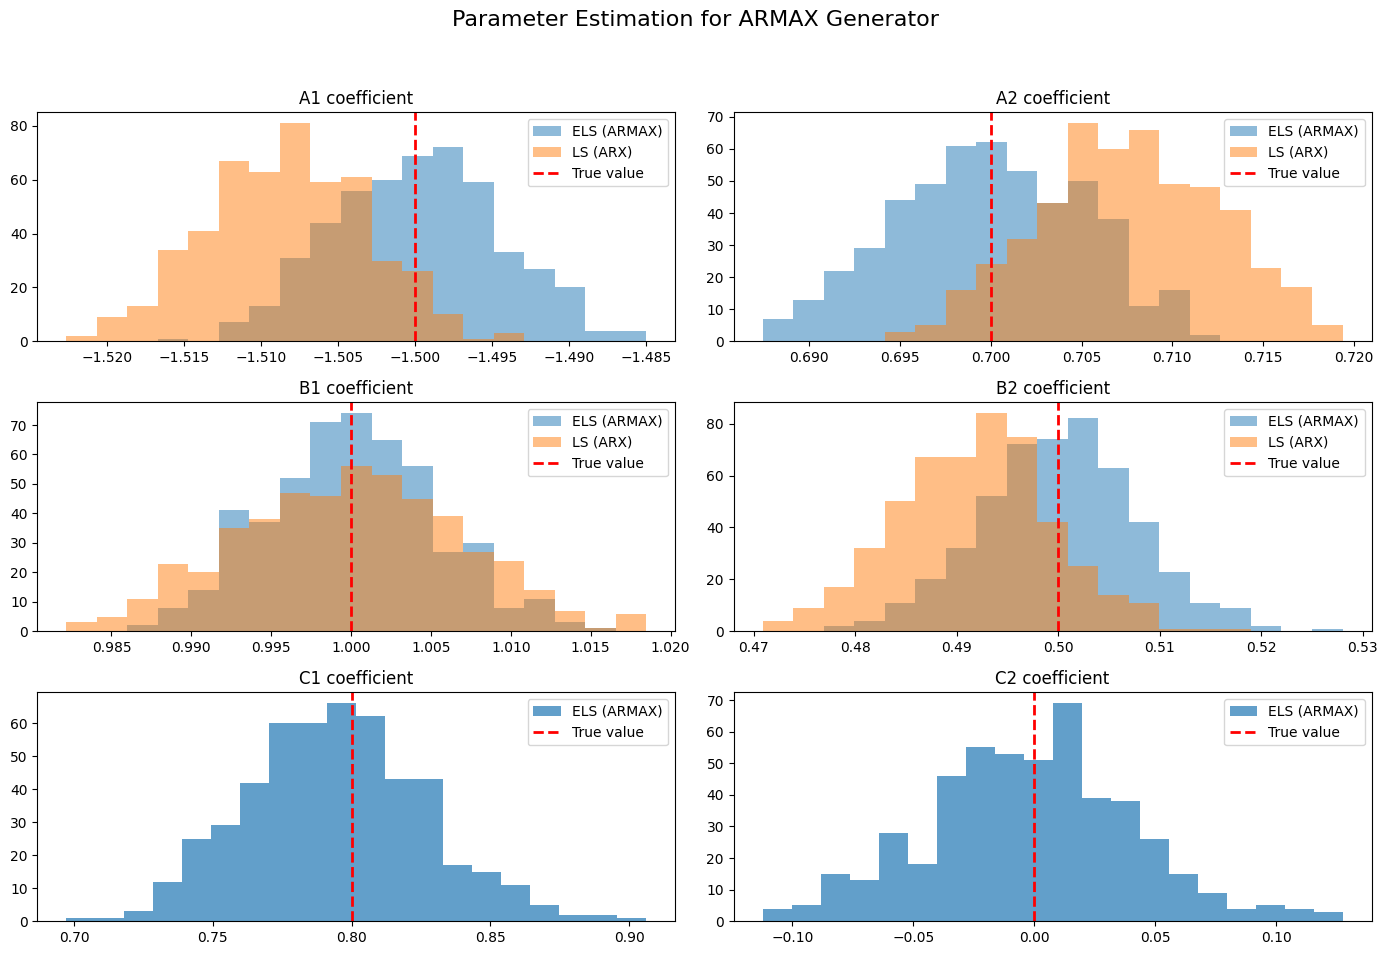
\includegraphics[width=\textwidth]{./imagens/parametros_armax.png}
    \caption{Histogramas dos coeficientes estimados pelos métodos MQ e MQE para o modelo ARMAX.}
    \label{fig:hist_armax}
\end{figure}

Para os coeficientes A e B, o método MQE é ligeiramente menos variável, e tem média significativamente mais próxima do valor real. Já para o coeficiente C, o método MQE é o único aplicável, dentre os dois, e apresenta média próxima do valor real, mas com variabilidade superior à dos coeficientes A e B.

A figura \ref{fig:hist_oe} mostra os histogramas dos coeficientes estimados pelos métodos MQ e MQE para o modelo OE. 

\begin{figure}[H]
    \centering
    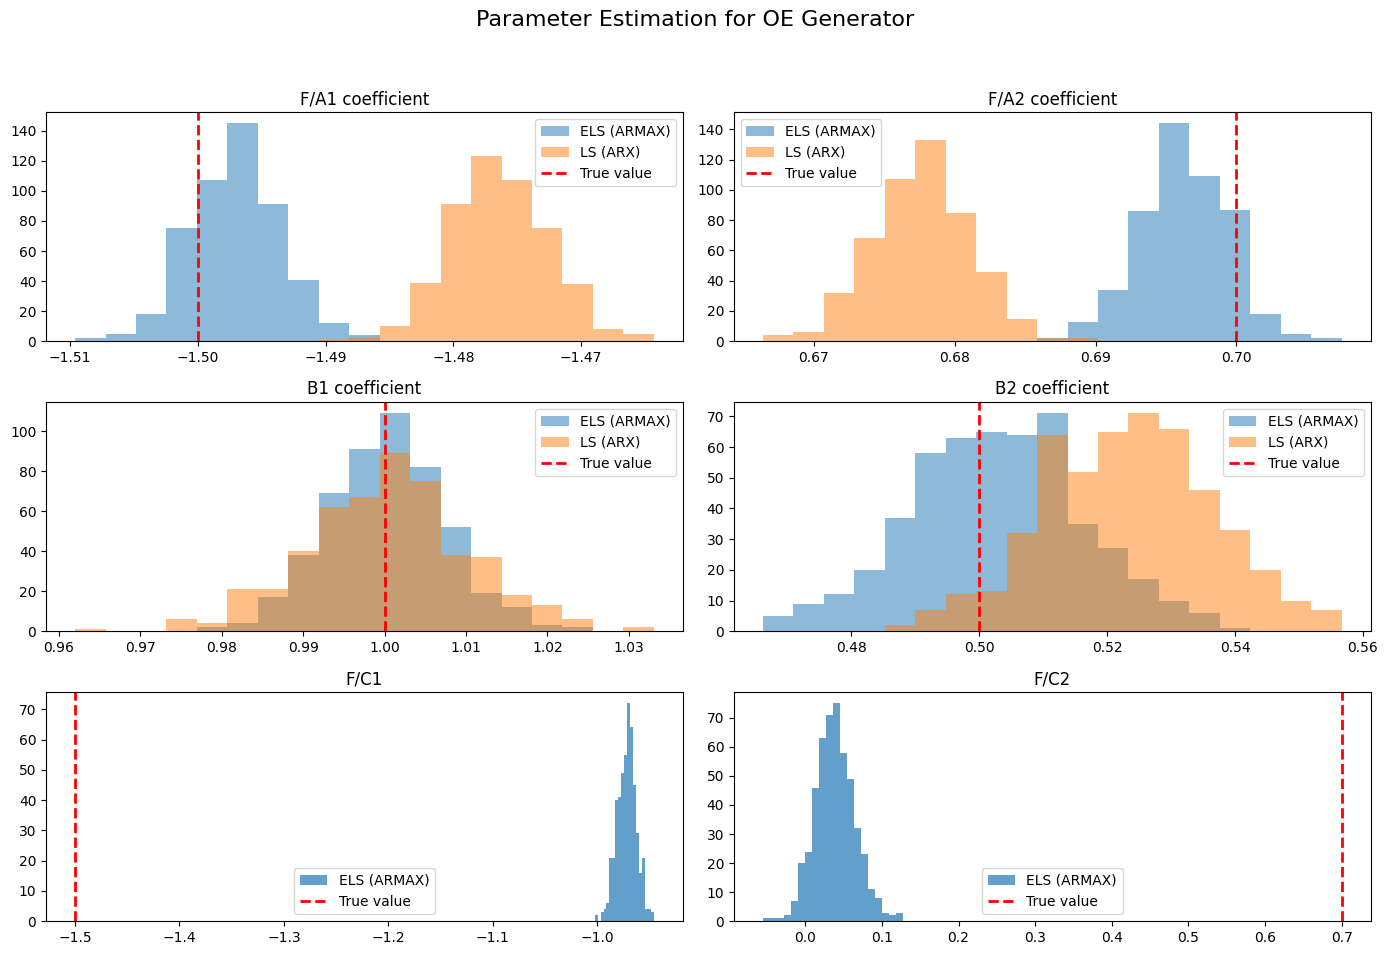
\includegraphics[width=\textwidth]{./imagens/parametros_oe.png}
    \caption{Histogramas dos coeficientes estimados pelos métodos MQ e MQE para o modelo OE.}
    \label{fig:hist_oe}
\end{figure}

Para os coeficientes F/A e B, o método MQE é igualmente variável ao método MQ, e tem média significativamente mais próxima do valor real, ainda que enviesada para o coeficiente de regressão das saídas. Já para o coeficiente F/C, o método MQE é fortemente enviesado, com média distante do valor real.

\section*{Questão 2}

\subsection*{E7.1}

Seja o ruído ARMA

\begin{equation}
    e[k] = E_1 e[k-1] + w[k] + W_1 w[k-1]
\end{equation}

o modelo MA

\begin{equation}
    y[k] = b_1 u[k-1] + b_2 u[k-2] + e[k]
\end{equation}

e o estimador MQ

\begin{equation}
    \hat{\Theta} = ( \Psi^T \Psi )^{-1} \Psi^T Y
\end{equation}

Como $\Psi$ não depende de $e[k]$, o estimador é não polarizado.

\subsection*{E7.2}

Para a matriz de covariância do ruído branco, o número de condição é 1, enquanto para a matriz de covariância do AM(1), o número de condição é $\approx 0.033$, calculado conforme sugerido no enunciado. Tal resultado indica que a matriz de covariância do AM(1) é mais próxima de ser singular do que a do ruído branco, o que pode levar a problemas numéricos na estimação dos parâmetros. Isso é esperado, uma vez que o ruído AM(1) apresenta correlação temporal, o que aproxima seus vetores de serem linearmente dependentes.

\subsection*{E7.3}

Seja

\begin{equation}
    y[k] = ay[k-1] + bu[k-1] + bw[k] + c\nu[k]
\end{equation}

onde $w$ é o ruído no atuador e $\nu$ é o ruído no sensor. Tomando $e = bw[k] + c\nu[k]$, temos

\begin{equation}
    y[k] = ay[k-1] + bu[k-1] + e[k]
\end{equation}

Se $u$ é conhecido, como no caso do ruído no sensor, o estimador EMQ é não polarizado. Entretanto, se $u[k] + w[k]$ é o valor medido, a entrada do sistema não é conhecida, precisa ser estimada, e o estimador é polarizado.

\end{document}